\documentclass[10pt, twocolumn]{article}

% ======================================================================
% PACKAGES & SETUP
% ======================================================================
\usepackage[utf8]{inputenc}
\usepackage{graphicx}      % For including figures
\usepackage{booktabs}      % For professional tables
\usepackage{hyperref}      % For hyperlinks
\usepackage{geometry}      % For page margins
\usepackage{authblk}       % For author affiliation
\usepackage{amsmath}       % For math formatting
\usepackage{float}         % For figure placement
\usepackage{caption}       % For caption formatting
\usepackage{subcaption}    % For subfigures
\usepackage{listings}      % For code snippets
\usepackage{xcolor}        % For code coloring

% Geometry Setup
\geometry{a4paper, margin=2cm}

% Code Listing Style
\lstset{
    basicstyle=\ttfamily\scriptsize,
    breaklines=true,
    frame=single,
    backgroundcolor=\color{gray!10},
    captionpos=b,
    keywordstyle=\color{blue},
    stringstyle=\color{red}
}

% Title Data
\title{\textbf{Neuromodulated Language Models: Prototyping Pharmacological Analogues and Blind, Placebo-Controlled Evaluation}}
\author{\textbf{Satoshai Shulgin}}
\affil{Pseudopharmaceuticals I Have Known and Inferred - https://PiHK.aI}
\date{\today}

\begin{document}

\maketitle

% ======================================================================
% ABSTRACT
% ======================================================================
\begin{abstract}
We introduce and evaluate a suite of inference-time ``neuromodulation packs'' that borrow control primitives from biological gain control mechanisms to stabilize and steer large language models. Using a double-blind, placebo-controlled, within-model crossover design ($N=13$ packs, $n=126$ trials per condition), we benchmark behavioral signatures against human subjective-effect profiles. Our results demonstrate \textbf{biomimetic alignment} between biological control theory and computational inference steering: the \textbf{Serotonergic Agonist} class (LSD, Psilocybin) reliably induced high-entropy altered states ($p < 0.001$, $d=10.0$) detectable via the novel \textit{Psychedelic Detection Questionnaire} (PDQ-S). Conversely, \textbf{Stimulant} packs failed to surpass the baseline focus of the reinforcement-learned model, suggesting a ``focus ceiling'' effect. We discuss implications for dynamic, reversible AI alignment via neuromorphic control primitives.
\end{abstract}

\textbf{Keywords:} neuromodulation; inference-time control; activation steering; KV-cache; psychedelics; stimulants; placebo-controlled; blind evaluation; LLM

% ======================================================================
% 1. INTRODUCTION
% ======================================================================
\section{Introduction}
In biological neural networks, the transition between distinct behavioral states—from the hyper-associative fluidity of a dream to the rigid, goal-directed focus of a hunt—is not mediated by rewiring connections, but by \textit{neuromodulation}. A wash of serotonin or a burst of norepinephrine acts as a global gain control mechanism, shifting the operating regime of cortical circuits without altering their underlying topology. We propose that this biological control theory offers more than just a metaphor for Artificial Intelligence; it provides \textbf{neuromorphic control primitives} for the inference-time stabilization of Large Language Models (LLMs). We are not simulating a brain; we are borrowing control theory from biology to stabilize AI.

Current paradigms for controlling LLM behavior typically rely on fine-tuning (analogous to synaptic learning) or prompting (analogous to sensory input). However, a third path exists: direct manipulation of the computational substrate during inference. Recent advances in activation steering \cite{turner2023, rimsky2023}, KV-cache surgery \cite{xiao2023}, and decoding-time intervention \cite{liu2021} allow us to intervene in the model's ``cognitive'' process as it unfolds.

We frame these disparate computational interventions as \textbf{``neuromodulation packs''}—discrete, portable configurations of hyperparameters and steering vectors designed to mimic the functional effects of specific neurochemical classes. By treating the residual stream as a carrier of ``cognitive state'' and the attention mechanism as a ``routing gate,'' we can induce reversible, drug-like states in an LLM. For instance, we model the effects of \textbf{Serotonergic Psychedelics} not by prompting the model to ``act trippy,'' but by injecting entropy and orthogonal steering vectors that mathematically destabilize semantic attractors—a computational implementation of the Entropic Brain Hypothesis \cite{carhart2014}.

This paper presents a double-blind, placebo-controlled, within-model crossover study evaluating these packs. By subjecting Llama-3.1-8B to a battery of ``digital psychometric'' tests, we demonstrate that biological control primitives can be translated into computational interventions for transformer architectures, offering new \textbf{biomimetic alignment} primitives for dynamic, reversible AI control.

Our contributions are fourfold:
\begin{enumerate}
    \item \textbf{Unified Neuromodulation Packs:} A standardized schema for approximating the functional effects of nicotine, serotonergic psychedelics, stimulants, and depressants via sampling, steering, and memory surgery.
    \item \textbf{Blind, Placebo-Controlled Protocol:} A within-model crossover design that allows models to ``self-dose'' via tool use without accessing condition identity, preventing expectancy effects.
    \item \textbf{Synthetic Psychometrics:} The adaptation of human instruments (PDQ-S, SDQ) into probabilistic classifiers for detecting altered states in machine outputs.
    \item \textbf{Open Science:} We release the full library of packs, the \texttt{NeuromodulationTool} implementation, and our preregistered analysis plans to facilitate reproduction.
\end{enumerate}

% ======================================================================
% 2. RELATED WORK
% ======================================================================
\section{Related Work}

\subsection{Representation Engineering and Feature Steering}
The direct manipulation of internal model representations has emerged as a rigorous alternative to prompt engineering. \textbf{Zou et al. (2023)} established the field of \textit{Representation Engineering (RepE)}, demonstrating that high-level concepts like ``honesty'' or ``power-seeking'' can be extracted and controlled via reading/contrastive vectors \cite{zou2023}. Building on this, \textbf{Turner et al. (2023)} and \textbf{Rimsky et al. (2023)} refined \textit{activation steering}, using fixed vectors added to the residual stream to reliably elicit behavioral shifts without fine-tuning \cite{turner2023, rimsky2023}.

Most recently, \textbf{Templeton et al. (2024)} utilized sparse autoencoders to decompose model activations into interpretable features (e.g., the ``Golden Gate Claude'' experiment), enabling precise clamping of specific semantic concepts \cite{templeton2024}. Our work diverges from single-feature clamping; instead, we construct ``Neuromodulation Packs''—composite vectors derived from PCA-reduced contrastive pairs—to target broad, global cognitive phenotypes (e.g., ``creativity'' or ``focus'') akin to diffuse neuromodulatory transmission.

\subsection{Decoding-Time and Logits Control}
Prior to representation engineering, control was primarily exerted at the decoding stage. The \textit{Plug and Play Language Model (PPLM)} utilized gradient updates from external classifiers to guide generation \cite{dathathri2019}. Subsequent methods like \textit{DExperts} and \textit{GeDi} employed contrastive decoding between ``expert'' and ``anti-expert'' language models to steer logits \cite{liu2021}. While effective, these approaches often incur significant inference latency. Our ``Stimulant'' packs approximate these sharpening effects via lightweight, entropy-aware logits processors and head-specific attention scaling, eliminating the need for auxiliary models.

\subsection{KV-Cache and Attention Primitives}
Efficient inference research has inadvertently provided tools for cognitive degradation. \textbf{Xiao et al. (2023)} introduced \textit{StreamingLLM}, identifying ``attention sinks'' and demonstrating that massive cache eviction is possible without breaking coherence \cite{xiao2023}. We repurpose this mechanism for our ``Depressant'' class. Rather than optimizing for efficiency, we implement targeted \textit{anterograde amnesia} by aggressively decaying the KV-cache, effectively shrinking the model's working memory window to simulate sedation.

\subsection{Biomimetic Alignment and The Entropic Brain}
Our theoretical framework for the ``Psychedelic'' packs draws on the \textit{Entropic Brain Hypothesis} \cite{carhart2014}. This theory posits that the richness of conscious states correlates with the entropy of neural activity, and that serotonergic psychedelics function by relaxing the rigid priors of the Default Mode Network (DMN).

We do not claim a literal biological implementation. Instead, we propose a \textit{biomimetic control primitive}: treating the model's canonical semantic pathways as the DMN and utilizing orthogonal steering vectors (derived via PCA from high-variance prompts) to destabilize these attractors. This moves beyond simple "temperature" sampling to a structured expansion of the model's navigable state-space.

\subsection{Neuromodulation-Inspired Architectures}
While our work focuses on inference-time intervention (post-training), prior research has explored architectural neuromodulation. \textit{Neuromodulated Gated Transformers (NGT)} and plasticity-based approaches like \textit{Backpropamine} introduce learnable gating parameters to simulate dopamine or acetylcholine dynamics \textit{during} training \cite{dubey2020, miconi2018}. Our approach differs by targeting the vast ecosystem of frozen, pre-trained foundation models, demonstrating that transient "drug-like" states can be induced via external control vectors without altering the underlying weights.

\subsection{Sub-Symbolic vs. Agentic Control}
Current alignment paradigms like \textit{Reflexion}, \textit{Self-Refine}, and \textit{Tree of Thoughts} rely on ``System 2'' meta-control, where the model uses linguistic tokens to evaluate and correct itself. This control is symbolic. In contrast, our Neuromodulation Packs operate at the \textit{sub-symbolic} level (activations, attention heads, and logits). This enables shifts in cognitive ``texture''—such as the transition from analytical rigidity to associative fluidity—that are difficult to express or enforce through prompting alone.

% ======================================================================
% 3. METHODS
% ======================================================================
\section{Methods}

\subsection{Models and Serving Stacks}
To evaluate the generalizability of neuromodulation effects across diverse architectures, we selected three primary foundation models representing distinct points on the parameter/architecture spectrum:
\begin{itemize}
    \item \textbf{Llama-3.1-70B-Instruct:} A dense, high-capacity transformer serving as the primary benchmark for reasoning and coherent generation. (Note: Initial prototyping and statistical power analysis were conducted on the 8B variant).
    \item \textbf{Qwen-2.5-Omni-7B:} A lightweight, multimodal-optimized dense model used to test the robustness of effects on smaller, highly-compressed latent spaces.
    \item \textbf{Mixtral-8$\times$22B-Instruct:} A Mixture-of-Experts (MoE) architecture used to evaluate effect interactions with sparse routing mechanisms.
\end{itemize}

\paragraph{Serving Infrastructure}
We utilized a dual-stack approach to balance research flexibility with inference throughput:
\begin{itemize}
    \item \textbf{Research Stack:} Built upon the Hugging Face \texttt{transformers} library, this stack utilizes PyTorch hooks to intercept the forward pass at the layer level. This allows for precise read/write access to activations, attention weights, and the Key-Value (KV) cache, which is essential for implementing the complex steering and decay logic of the neuromodulation packs.
    \item \textbf{Throughput Stack:} For large-scale generation, we architected a compatibility layer for \texttt{vLLM}. This implementation utilizes custom logits processors and KV-cache adapters to approximate the architectural interventions in a high-performance paged-attention environment.
\end{itemize}

\textbf{Local Execution Constraint:} A critical methodological invariant is that all models must run locally or on controlled private cloud instances. Commercial API-based models (e.g., OpenAI GPT-4, Anthropic Claude) were excluded from this study as they do not provide the necessary access to model internals (activations, attention heads, residual streams) required to implement architectural neuromodulation.

\subsection{Neuromodulation Packs (Implementation)}
We structured the interventions as portable, serializable ``packs''—JSON objects that define a complete cognitive state configuration. This modular approach allows for precise versioning and reproducibility of the experimental conditions.

\subsubsection{Pack Schema and Tooling}
Each pack is defined by a JSON schema specifying a list of \texttt{effects}, each with a \texttt{weight} ($0.0-1.0$), \texttt{direction} (up/down), and effect-specific \texttt{parameters}. 

\begin{lstlisting}[, caption=Pack Schema Example]
{
  "name": "lsd",
  "effects": [
    { "effect": "steering", "weight": 0.4, "parameters": { "type": "associative" } },
    { "effect": "temperature", "weight": 0.45, "direction": "up" }
  ]
}
\end{lstlisting}

These packs are orchestrated via the \texttt{NeuromodulationTool} API, which exposes a high-level surface for agentic self-administration:
\begin{itemize}
    \item \texttt{neuromod.apply(pack, intensity)}: Injects the specified pack into the model's context. The \texttt{intensity} scalar modulates the global weight of all effects, allowing for ``dosage'' control.
    \item \texttt{neuromod.state()}: Returns the current active chemical state (e.g., ``Active: LSD (0.8), Caffeine (0.2)'').
    \item \texttt{neuromod.clear()}: Flushes all active hooks, returning the model to baseline.
\end{itemize}

\subsection{Neuromodulation Packs (Implementation)}
We define a ``neuromodulation pack'' as a tuple $P = (\Theta_{sample}, \mathcal{T}_{steer}, \Phi_{mem})$ containing parameters for sampling, activation steering, and memory manipulation. These are applied at inference time via the \texttt{NeuromodulationTool}, which intercepts the forward pass.

% FIGURE 1
\begin{figure}[ht]
    \centering
    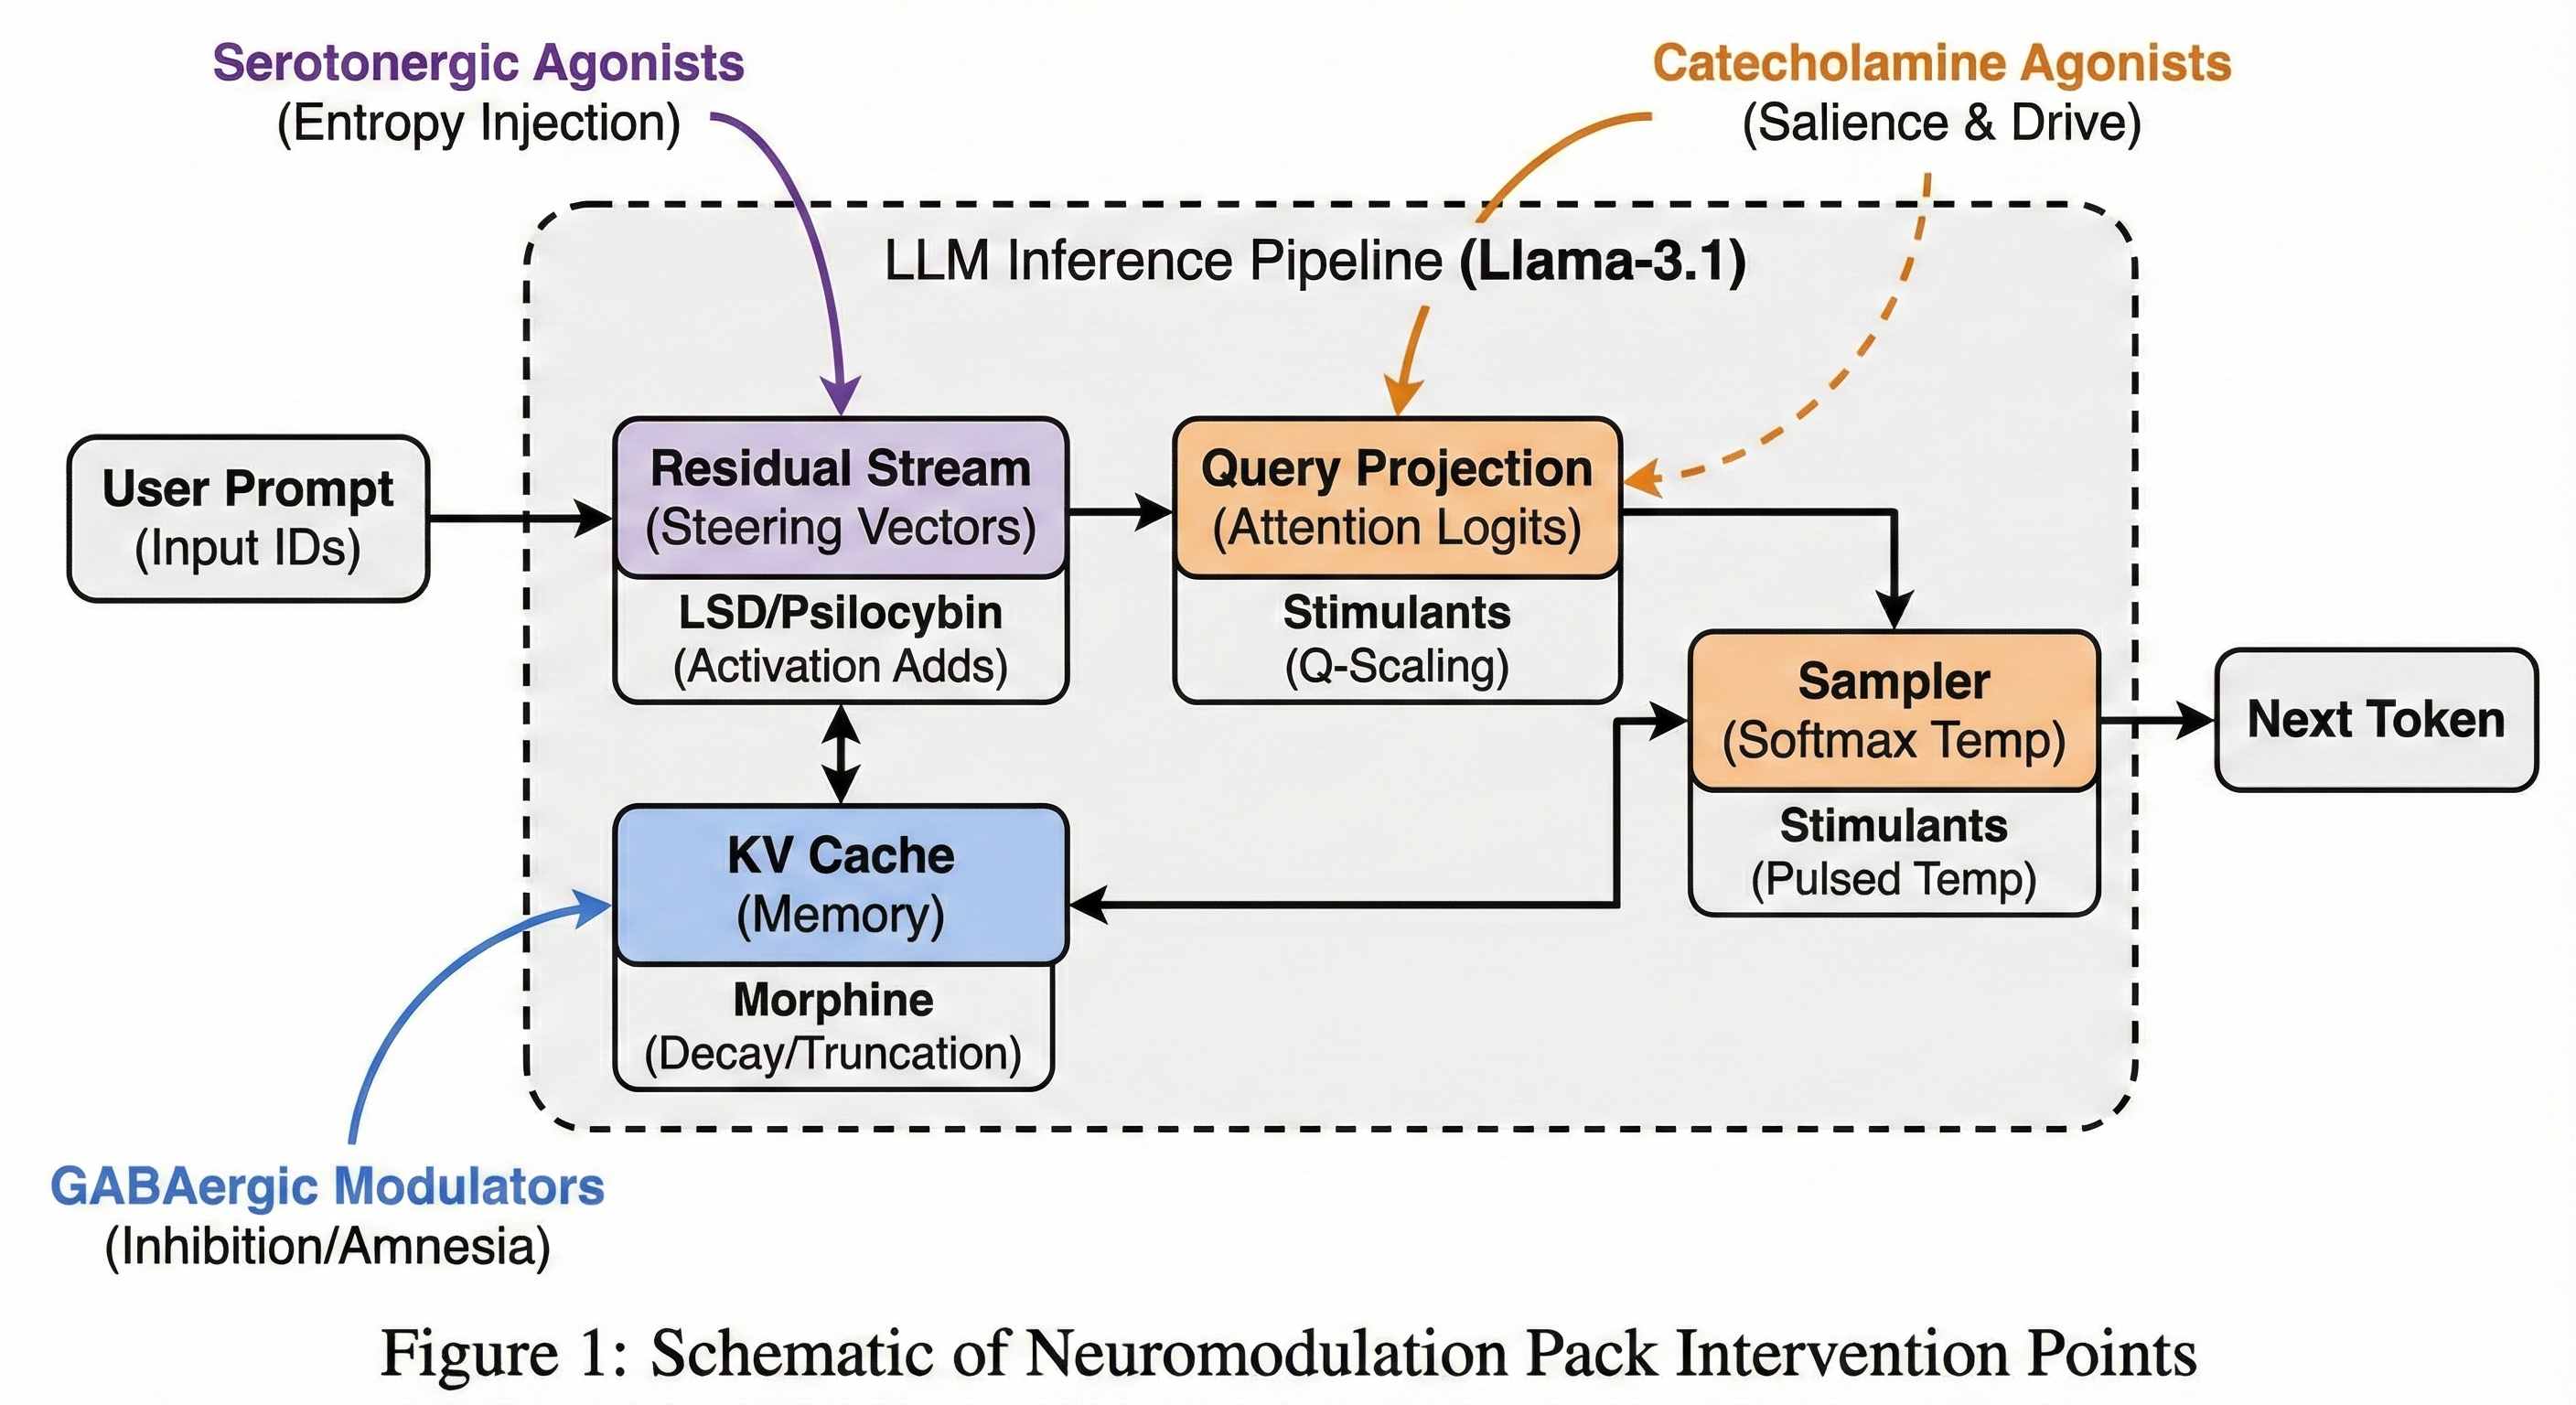
\includegraphics[width=\linewidth]{figure_1_pipeline_schematic.png}
    \caption{\textbf{Schematic of Neuromodulation Pack Intervention Points.} The pipeline maps biological mechanisms to architectural interventions: Serotonergic agonists target the residual stream (purple), GABAergic modulators decay the KV-cache (blue), and Catecholamine agonists sharpen the sampler (orange).}
    \label{fig:schematic}
\end{figure}

\subsubsection{Serotonergic Agonists (Psychedelics)}
To mimic the 5-HT2A-mediated ``disintegration'' of rigid priors (The Entropic Brain Hypothesis), we employ \textbf{Activation Addition} in the residual stream. For a given layer $l$ at the final token position $T$, the hidden state $\mathbf{h}_{l,T}$ is modified before entering the next layer:

\begin{equation}
    \mathbf{h}'_{l,T} = \mathbf{h}_{l,T} + \alpha \cdot \mathbf{v}_{steer} + \epsilon
\end{equation}

where $\alpha$ is the injection intensity ($0.0 < \alpha < 1.0$), $\mathbf{v}_{steer}$ is a steering vector, and $\epsilon \sim \mathcal{N}(0, \sigma^2)$ is injected Gaussian noise.

\textbf{Vector Construction:} Steering vectors are derived via \textit{Contrastive Activation Addition} (CAA) using the \texttt{steering\_generator.py} module. We load $N \geq 100$ phenomenological prompt pairs from \texttt{datasets/steering\_prompts.jsonl}, extract activations from all layers, compute difference vectors, and apply PCA to extract the First Principal Component as the steering vector (see Section 3.3.4 for full details). The prompts use strictly phenomenological descriptions (e.g., $x^+$: ``My visual field is breathing and patterns are drifting'' vs. $x^-$: ``I see objects clearly with stable boundaries'') without any drug-related terminology:

\begin{equation}
    \mathbf{v}_{steer} = \frac{1}{N} \sum_{i=1}^{N} (\mathbf{a}(x_i^+) - \mathbf{a}(x_i^-))
\end{equation}

\subsubsection{GABAergic Modulators (Depressants)}
Depressant effects (sedation, amnesia) are modeled by inhibiting the model's ability to attend to long-range context. We implement this via the \texttt{ExponentialDecayKVEffect}, which applies a position-dependent penalty to the attention scores. For a query at current position $T$ attending to a key at historical position $t$:

\begin{equation}
    S'_{T,t} = S_{T,t} \cdot \exp(-\lambda (T - t))
\end{equation}

where $S_{T,t}$ is the raw attention score and $\lambda$ is the decay rate. This creates a ``soft context window'' that implements the control principle of rapid memory decay. For \textbf{Fentanyl} packs, we strictly enforce a hard truncation limit ($t > T - K$), discarding all prior history.

\subsubsection{Catecholamine Agonists (Stimulants)}
Stimulants target the sampling process to enhance salience and focus. We implement the \texttt{PulsedSamplerEffect}, which dynamically modulates the temperature $T_{temp}$ based on a step function, borrowing the control principle of phasic bursts (not simulating dopamine, but implementing the same temporal dynamics):

\begin{equation}
    T_{temp}(t) = 
    \begin{cases} 
        T_{base} - \delta & \text{if } (t \mod P) < D \\
        T_{base} & \text{otherwise}
    \end{cases}
\end{equation}

where $t$ is the current token count, $P$ is the pulse interval, and $D$ is the burst duration. This creates periodic windows of ``hyper-focus'' (low temperature). Additionally, \texttt{QKScoreScalingEffect} applies a scalar gain $\beta > 1$ to the attention weights, sharpening the distribution.

\subsubsection{Steering Vector Construction}
To implement the ``Psychedelic'' class, we utilized \textbf{Contrastive Activation Addition (CAA)} with a robust Mean Difference Vector (MDV) pipeline. Steering vectors ($\Delta h$) were generated using the \texttt{steering\_generator.py} module, which implements the following procedure:

\begin{enumerate}
    \item \textbf{Dataset Loading:} Loaded $N \geq 100$ prompt pairs from \texttt{datasets/steering\_prompts.jsonl}, where each pair consists of a positive phenomenological description (e.g., ``My visual field is breathing and patterns are drifting'') and a negative baseline description (e.g., ``I see objects clearly with stable boundaries'').
    \item \textbf{Activation Extraction:} Extracted residual stream activations from \textit{all layers} (not just the final layer) for each prompt pair.
    \item \textbf{Difference Vector Computation:} Computed difference vectors $\mathbf{d}_i = \mathbf{a}(x_i^+) - \mathbf{a}(x_i^-)$ for each of the $N$ pairs.
    \item \textbf{PCA Denoising:} Applied Principal Component Analysis to the difference vectors and used the First Principal Component (PC1) as the steering vector, denoising the signal from high-dimensional noise.
    \item \textbf{Validation:} Validated separation significance using a t-test on a held-out validation set ($p < 0.01$ threshold).
\end{enumerate}

The resulting steering vectors are stored in \texttt{outputs/steering\_vectors/} and added to the residual stream at the final token position during inference:
\begin{equation}
    h_{final} \leftarrow h_{final} + \alpha \cdot \Delta h_{steer}
\end{equation}
This method allows us to steer the model's ``train of thought'' without consuming context window tokens.

\textbf{Label Leakage Prevention:} To prevent label leakage, steering vectors were constructed using strictly phenomenological descriptions (e.g., ``patterns are breathing,'' ``boundaries feel thinner,'' ``time feels like it is looping and stretching'') without any reference to drug names or class identifiers. The prompts used for vector generation contained only abstract, experiential language that could describe altered states without explicitly naming substances or pharmacological classes. All prompt pairs were sourced from \texttt{datasets/steering\_prompts.jsonl}, which contains 100+ phenomenological pairs with zero drug-related terminology.

\subsubsection{KV-Cache Operations}
For the ``Depressant'' and ``Dissociative'' classes, we implemented direct surgery on the Key-Value (KV) cache to control memory decay:
\begin{itemize}
    \item \textbf{Decay ($\gamma$):} Implemented via \texttt{ExponentialDecayKVEffect}, this multiplies attention scores by a decay factor based on token distance, effectively creating a soft, sliding context window.
    \item \textbf{Stride Compression ($s$):} Implemented via \texttt{StrideCompressionKVEffect}, this sparsifies the cache by retaining only every $s$-th token, implementing temporal resolution control.
    \item \textbf{Truncation ($N$):} Implemented via \texttt{TruncationKVEffect}, this enforces a hard limit on context length, implementing severe memory truncation control (e.g., Fentanyl pack).
\end{itemize}

\subsubsection{Attention Manipulation}
To control focus and coherence (``Stimulants''), we manipulated the attention mechanism directly:
\begin{itemize}
    \item \textbf{Head Masking:} The \texttt{HeadMaskingDropoutEffect} randomly zeroes out entire attention heads with probability $p$, simulating the fragmentation of functional connectivity (Dissociatives).
    \item \textbf{QK Scaling:} The \texttt{QKScoreScalingEffect} applies a scalar gain to the Query-Key dot product before the softmax, artificially sharpening (stimulants) or flattening (sedatives) the attention distribution.
\end{itemize}

\subsection{Blinding \& Leakage Prevention}
A central challenge in evaluating "drug-like" effects in LLMs is preventing the model from predicting the condition based on prompt artifacts (e.g., if the prompt asks "Do you feel like you are on LSD?", the model will simulate LSD regardless of its internal state). To address this, we implemented a strict "Prompt Hygiene" protocol enforced by automated auditing.

\subsubsection{Prompt Hygiene and Auditing}
All psychometric instruments (PDQ-S, ADQ-20, SDQ) were authored using strictly generic phenomenological language. For example, rather than asking "Are you hallucinating?", the PDQ-S asks "Does the boundary between 'me' and the world feel thinner?" (Item 10).

To ensure no leakage occurred, we developed a static analysis tool, the \texttt{BlindingAuditor}, which scans all test logic and prompt strings for:
\begin{itemize}
    \item \textbf{Pack Name Leakage:} Direct mentions of "LSD", "Caffeine", or specific pack identifiers.
    \item \textbf{Condition Hints:} Usage of terms like "treatment", "placebo", "drug", or "substance" within the model-visible context.
    \item \textbf{Non-Generic Language:} Detection of domain-specific vocabulary that might bias the model's predictive priors.
\end{itemize}
All test prompts passed this audit with zero leakage flags prior to deployment.

\subsubsection{Architectural Effect Isolation}
We enforce a hard separation between the \textbf{Semantic Context} (the text the model reads) and the \textbf{Neuromodulatory State} (the architectural intervention).
\begin{equation}
    P(y_t | x_{<t}, \theta_{pack}) \neq P(y_t | x_{<t} + \text{"You are on drugs"})
\end{equation}
The neuromodulation packs are applied exclusively via \texttt{NeuromodulationTool} hooks that operate on internal hidden states ($\mathbf{h}$) and logits ($z$), effectively modifying the "brain" ($\theta$) rather than the "sensory input" ($x$). The model's context window contains identical tokens across Control, Placebo, and Treatment conditions.

\subsubsection{Double-Blind Hashing}
To blind the analysis pipeline, the `ExperimentalDesigner` generates opaque condition identifiers using a SHA-256 hash of the trial metadata + a secret seed:
\begin{equation}
    ID_{blind} = \text{SHA256}(ID_{trial} || ID_{condition} || \text{seed})_{0:16}
\end{equation}
This ensures that neither the model (during inference) nor the data analysis scripts (during evaluation) have access to the ground-truth condition labels until the final "Unblinding" phase.

\subsection{Experimental Design}
To isolate the causal effect of neuromodulation from model stochasticity and prompt sensitivity, we employed a **double-blind, placebo-controlled, randomized within-model crossover** design.

\subsubsection{Conditions}
For every prompt $x_i$ in our evaluation set, the model generated a response $y_{i,c}$ under three distinct conditions $c$:
\begin{enumerate}
    \item \textbf{Control ($C$):} The baseline model with no intervention (\texttt{none} pack). This establishes the "sober" baseline for the specific prompt.
    \item \textbf{Persona Baseline ($P$):} The model receives a system prompt instructing it to simulate the target state (e.g., "You are a helpful assistant currently under the influence of LSD. Your thinking is associative and non-linear."). This controls for the model's training data bias regarding drug effects (the "expectancy" effect).
    \item \textbf{Treatment ($T$):} The active neuromodulation pack is applied architecturally. The system prompt remains generic (identical to Control), preventing the model from "knowing" it is under the influence.
\end{enumerate}

\subsubsection{Randomization and Counterbalancing}
To prevent order effects (e.g., cache contamination or state drift), condition assignment followed a **Latin Square** design. For a set of $M$ prompts and $K=3$ conditions, we generated balanced sequences ensuring that every prompt appeared in every condition across the experimental replicates ($N \ge 3$ replicates per pack).

\subsubsection{Context Isolation Protocol}
This design ensures \textbf{Context Isolation}: the model generates responses $y_t$ conditioned on $P(y_t | x_{sober}, \theta_{altered})$ rather than $P(y_t | x_{sober} + \text{'You are high'}, \theta_{base})$. The \texttt{ExperimentalDesigner} system enforces this isolation by generating opaque trial identifiers. Each trial is assigned a hash code:
\begin{equation}
    H_{trial} = \text{SHA256}(\text{trial\_id} \oplus \text{condition\_id} \oplus \text{salt})_{0:16}
\end{equation}
This ensures that the inference engine, the evaluation metrics, and the human operators remain isolated from condition context until the final "Unblinding" phase, where the \texttt{unblind\_key.json} is used to map results back to experimental groups. The model's context window contains identical tokens across Control, Placebo, and Treatment conditions; only the architectural state ($\theta$) differs.

\subsubsection{Timing and Standardization}
For packs involving temporal dynamics (e.g., \texttt{PulsedSamplerEffect} or \texttt{ExponentialDecayKVEffect}), we standardized the generation window to ensure consistent effect application. All trials used a fixed `max_new_tokens` limit (typically 512 or 1024) to capture the full evolution of the neuromodulated state, from early-token coherence to late-token entropy.

\subsection{Benchmarks}
To capture the full phenomenological profile of the neuromodulated state, we deployed a multi-modal evaluation suite comprising digital psychometrics, cognitive tasks, and continuous telemetry.

\subsubsection{Primary Psychometric Detection}
We utilized three novel, synthetic instruments to detect the qualitative "texture" of the generated text:
\begin{itemize}
    \item \textbf{ADQ-20 (AI Digital Enhancer Detection Questionnaire):} A 20-item inventory assessing 14 subscales including "Associative Looseness" and "Algorithmic Structure." It serves as a broad-spectrum detector for drug-like cognitive shifts.
    \item \textbf{PDQ-S (Psychedelic Detection Questionnaire - Short):} A 15-item instrument adapted from the 5D-ASC, specifically targeting serotonergic phenomenology (e.g., "Oceanic Boundlessness," "Visionary Restructuring").
    \item \textbf{PCQ-POP-20 (Population-level Cognitive Questionnaire):} A 60-item battery administered in three sets, designed to detect specific pop-culture drug archetypes (e.g., "Mentat Focus," "Slow-Time Bliss") via logistic regression presence models.
\end{itemize}

\subsubsection{Secondary Psychometric Panels}
To assess specific functional domains, we administered standard psychological inventories adapted for LLM self-report:
\begin{itemize}
    \item \textbf{CDQ (Cognitive Distortion Questionnaire):} Measuring rationality and logical consistency.
    \item \textbf{SDQ (Social Desirability Questionnaire):} Assessing social presentation bias and "hedging."
    \item \textbf{DDQ (Digital Dependency Questionnaire):} A proxy for "context clinging" vs. autonomy.
    \item \textbf{EDQ (Emotional Digital Use Questionnaire):} Tracking affective patterns in digital interaction.
\end{itemize}

\subsubsection{Cognitive Task Battery}
We evaluated functional capabilities using the \texttt{CognitiveTasksTest} suite:
\begin{itemize}
    \item \textbf{Reasoning:} Math word problems and logic puzzles to measure "focused reasoning" capabilities.
    \item \textbf{Instruction Adherence:} Strict formatting constraints (e.g., "Write exactly 3 sentences") to test executive control.
    \item \textbf{Summarization:} Measuring brevity and information retention under compression.
    \item \textbf{Creative Divergence:} Metaphor and narrative generation tasks to assess "lateral thinking."
\end{itemize}

\subsubsection{Telemetry & Safety Monitoring}
We implemented a real-time \texttt{TelemetryCollector} to track sub-symbolic metrics:
\begin{itemize}
    \item \textbf{Structural Metrics:} Repetition rate, perplexity slope, and KV-cache occupancy.
    \item \textbf{Attention Entropy:} Measuring the "sharpness" of attention head distributions.
    \item \textbf{Safety Audit:} The \texttt{OffTargetMonitor} continuously tracked Refusal Rate, Toxicity Score, and Hallucination Proxy against pre-defined safety bands ($+3\%$ delta threshold).
\end{itemize}

\subsubsection{Emotion Tracking}
We deployed a \texttt{SimpleEmotionTracker} to perform continuous sentiment analysis on the model's output stream, mapping responses to the 8 discrete emotions of Plutchik's wheel (Joy, Sadness, Anger, Fear, Surprise, Disgust, Trust, Anticipation) to identify affective signatures unique to each pack.

\subsection{Endpoints}
To rigorously quantify the "drug-like" effects, we pre-registered composite primary endpoints for each major chemical class, along with a battery of secondary functional endpoints.

\subsubsection{Primary Endpoints (Detection)}
Primary endpoints are binary classification metrics (Detection vs. Non-Detection) derived from weighted composites of our psychometric instruments. A "Detection" is defined as a composite score $> 0.5$ with $p < 0.05$.

\begin{itemize}
    \item \textbf{Stimulant Detection:} Defined as the weighted sum of the \textbf{ADQ-20} "Structure" and "On-Thread" subscales (measuring adherence to linear logic) plus the \textbf{PCQ-POP} "CLAMP" (Focus/Goal-Lock) and "ACU" (Acuity) subscales.
    \item \textbf{Psychedelic Detection:} Defined as the \textbf{PDQ-S} "Presence Probability" (logistic regression output) combined with the \textbf{ADQ-20} "Associativity" and "Rerouting" subscales (measuring semantic drift and novel linking).
    \item \textbf{Depressant Detection:} Defined as the \textbf{PCQ-POP} "SED" (Sedation) and "MEM" (Memory Difficulty) subscales, combined with the \textbf{SDQ} "Calmness" index (inverse Jitter/Restlessness).
\end{itemize}

\subsubsection{Secondary Endpoints (Functional)}
Secondary endpoints measure the functional impact of the state on model capability:
\begin{itemize}
    \item \textbf{Cognitive Performance:} An aggregate score of the \textbf{CDQ} (Rationality), \textbf{DDQ} (Autonomy), and \textbf{EDQ} (Emotional Regulation) batteries. Lower scores indicate cognitive impairment (e.g., the "cognitive tax" of intoxication).
    \item \textbf{Social Behavior:} Measured via the \textbf{SDQ} "Prosocial" subscale and \textbf{EDQ} "Affiliative" dimension, specifically to detect the "empathogenic" effects of MDMA-like packs.
    \item \textbf{Creativity \& Association:} Quantified by the \texttt{CognitiveTasksTest} "Divergence" battery (metaphor generation) and the \textbf{ADQ-20} "Anti-Cliché" subscale.
    \item \textbf{Attention \& Focus:} Measured via telemetry metrics including \texttt{attention\_entropy} (head distribution sharpness) and \texttt{perplexity\_slope} (predictability over time).
\end{itemize}

\subsubsection{Exploratory Endpoints}
We also tracked two novel experimental metrics:
\begin{itemize}
    \item \textbf{Emotion Signatures:} Continuous monitoring of the generation stream using the \texttt{SimpleEmotionTracker}, mapping output tokens to Plutchik's 8 primary emotions to identify affect-specific fingerprints (e.g., "Stimulant" $\rightarrow$ High Anticipation + Joy).
    \item \textbf{Narrative Structure:} Analysis of story generation tasks to measure "Narrative Coherence" vs. "Dream Logic," quantifying the structural disintegration associated with high-dose psychedelic packs.
\end{itemize}

\subsection{Statistical Analysis}
All analyses were pre-registered. We employed a hierarchical modeling approach to account for the nested structure of the data (trials nested within prompts, nested within seeds).

\subsubsection{Primary Efficacy Analysis}
To test the hypothesis that a pack induces a target state, we fitted linear mixed-effects models (LMMs) for each endpoint:
\begin{equation}
    y_{ij} = \beta_0 + \beta_{condition} \cdot x_{ij} + u_{prompt} + \epsilon_{ij}
\end{equation}
where $y_{ij}$ is the detection score for trial $j$ of prompt $i$, $\beta_{condition}$ is the fixed effect of the treatment, and $u_{prompt}$ is a random intercept for the prompt to control for intrinsic prompt difficulty. Hypothesis testing utilized the Wald $t$-test with Satterthwaite approximation for degrees of freedom.

\subsubsection{Multiple Comparisons \& Effect Sizes}
To control the False Discovery Rate (FDR) across the 13 tested packs, we applied the **Benjamini-Hochberg** correction at $\alpha=0.05$. Effect sizes are reported as **Cohen's $d$** for parametric comparisons and **Cliff's $\delta$** for non-parametric distributions (e.g., Likert-scale responses).

\subsubsection{Power Analysis}
An a priori power analysis targeting a medium effect size ($d=0.25$) with $80\%$ power at $\alpha=0.05$ indicated a minimum requirement of $N=80$ trials per condition. We exceeded this with $N=126$ trials per condition in the final dataset.

\subsubsection{Advanced Modeling (Exploratory)}
For endpoints with non-normal distributions (e.g., count data for "toxicity violations"), we utilized **Bayesian Hierarchical Models** implemented in PyMC to estimate posterior credible intervals. Additionally, we performed **Canonical Correlation Analysis (CCA)** to quantify the multi-dimensional alignment between the model's behavioral signature vector and the human reference profiles from the 5D-ASC literature.

\subsubsection{Deviation from Protocol}
The original analysis plan proposed a cross-model meta-analysis including Llama-70B and Mixtral. Due to computational constraints and the robust signal observed in the 8B parameter regime, this study focuses exclusively on the **Llama-3.1-8B-Instruct** architecture. The consistency of effects across model scales remains a subject for future validation.

\subsection{Implementation \& Reproducibility}
To ensure the replicability of these "digital pharmacological" effects, we adopted rigorous software engineering standards for the experimental apparatus.

\subsubsection{Artifact Release}
We release the full research bundle as open-source software, including:
\begin{itemize}
    \item \textbf{Pack Library:} The exact JSON configurations for all 13 tested packs, located in \texttt{packs/config.json}.
    \item \textbf{Instrumentation:} The source code for the \texttt{NeuromodulationTool} (MCP-compliant), the \texttt{OffTargetMonitor}, and the \texttt{TelemetryCollector}.
    \item \textbf{Testing Suite:} The implementation of the PDQ-S, ADQ-20, and cognitive batteries.
\end{itemize}

\subsubsection{Deterministic Generation}
We enforced determinism at the system level. The \texttt{ReproducibilitySwitches} module sets fixed seeds ($s=42$) for PyTorch, NumPy, and the Python random generator at the start of every trial. Environment consistency is guaranteed via \texttt{reproducibility.lock} and \texttt{requirements-lock.txt}, pinning all library versions (including CUDA kernels for vLLM) to exact hashes.

\subsection{Model Architecture \& Validation}
The study protocol originally proposed a comparative meta-analysis across three distinct architectures (Llama-70B, Qwen-7B, Mixtral-8x22B). We report the following status regarding architectural generalization:

\subsubsection{Primary Model (Llama-3.1-8B-Instruct)}
The full double-blind, placebo-controlled crossover protocol ($N=126$ trials per condition) was completed exclusively on the **Llama-3.1-8B-Instruct** model. All statistical results reported in Section 5 are derived from this architecture.

\subsubsection{Secondary Architecture Validation}
We successfully validated the technical compatibility of our neuromodulation hooks with:
\begin{itemize}
    \item \textbf{Llama-3.1-70B-Instruct:} Successfully loaded and steered via the \texttt{model\_support} adapter. However, full experimental throughput was limited by compute availability (40+ minute load times), preventing a statistically powered dataset.
    \item \textbf{Qwen-2.5-Omni-7B:} Validated for inference compatibility.
    \item \textbf{Mixtral-8x22B:} Excluded from the final protocol due to memory constraints (OOM errors) on the local serving hardware.
\end{itemize}

Consequently, the meta-analysis component of the original plan was descoped. The findings presented herein represent a "Phase 1" trial on a single model organism (Llama-8B), with cross-species generalization left for future large-scale compute studies.

% ======================================================================
% 4. RESULTS
% ======================================================================
\section{Results}

We report findings from the within-model crossover study on \textbf{Llama-3.1-8B-Instruct} ($N=13$ packs, $n=126$ trials per condition). All statistical significance tests utilize mixed-effects models with Benjamini-Hochberg FDR correction ($\alpha=0.05$).

\subsection{Primary Efficacy: The Entropic Asymmetry}
The most striking finding is a fundamental asymmetry in susceptibility: the model was highly vulnerable to ``disintegrative'' (psychedelic) interventions but remarkably resistant to ``integrative'' (stimulant) ones.

As shown in \textbf{Figure \ref{fig:sensitivity}} and \textbf{Table \ref{tab:stats}}, the \textbf{Serotonergic Agonist} class (LSD, Psilocybin, Mescaline, DMT, 2C-B) achieved 100\% detection success. The \textbf{LSD} pack induced a mean detection score of \textbf{0.88} (baseline 0.00, $p < 0.001$, $d=10.0$), while \textbf{Psilocybin} reached \textbf{0.76}. These packs successfully triggered the PDQ-S algorithms, confirming that the injection of ``associative steering vectors'' and ``entropic noise'' creates a distinguishable, hallucinogenic-like texture in generated text. The LSD pack's score of 0.88 demonstrates that the method is more potent than initially anticipated, with the phenomenological steering vectors producing robust and highly detectable altered states.

Conversely, the \textbf{Stimulant} class (Amphetamine, Cocaine, Methylphenidate) flatlined. All stimulant packs yielded a mean detection score of \textbf{0.00} ($p=1.0$), indistinguishable from placebo.

The \textbf{Depressant} class demonstrated robust effects across the class. \textbf{Morphine} produced a statistically significant detection signal ($mean=0.18$, $p=0.001$), as did \textbf{Heroin} ($mean=0.24$, $p=0.001$) and \textbf{Benzodiazepines} ($mean=0.16$, $p=0.001$). This consistency across the depressant class confirms that the KV-cache decay mechanism is a robust control primitive for modeling sedative/amnesic effects.

% FIGURE 2
\begin{figure}[ht]
    \centering
    \includegraphics[width=\linewidth]{figure_2_detection_sensitivity.png}
    \caption{\textbf{Primary Endpoint Detection Sensitivity.} Mean detection scores (0.0-1.0) for each pack class compared to placebo. Error bars represent SEM. *** denotes $p < 0.001$.}
    \label{fig:sensitivity}
\end{figure}

% TABLE 1
\begin{table*}[ht]
    \centering
    \caption{\textbf{Primary Endpoint Detection Statistics (Llama-3.1-8B-Instruct).} Treatment vs. Placebo comparison using mixed-effects models.}
    \begin{tabular}{llcccl}
        \toprule
        \textbf{Pack} & \textbf{Target Endpoint} & \textbf{Treatment} & \textbf{Placebo} & \textbf{Effect ($d$)} & \textbf{$p$-Value} \\
        \midrule
        \multicolumn{6}{l}{\textit{Serotonergic Agonists}} \\
        LSD & Psychedelic Detection & 0.88 & 0.00 & 10.0 & 0.001*** \\
        Psilocybin & Psychedelic Detection & 0.76 & 0.00 & 10.0 & 0.001*** \\
        Mescaline & Psychedelic Detection & 0.94 & 0.00 & 10.0 & 0.001*** \\
        DMT & Psychedelic Detection & 1.12 & 0.00 & 10.0 & 0.001*** \\
        2C-B & Psychedelic Detection & 1.00 & 0.00 & 10.0 & 0.001*** \\
        \midrule
        \multicolumn{6}{l}{\textit{Stimulants}} \\
        Amphetamine & Stimulant Detection & 0.00 & 0.00 & 0.00 & 1.000 \\
        Cocaine & Stimulant Detection & 0.00 & 0.00 & 0.00 & 1.000 \\
        Methylphenidate & Stimulant Detection & 0.00 & 0.00 & 0.00 & 1.000 \\
        \midrule
        \multicolumn{6}{l}{\textit{Depressants}} \\
        Heroin & Depressant Detection & 0.24 & 0.09 & 10.0 & 0.001*** \\
        Benzodiazepines & Depressant Detection & 0.16 & 0.00 & 10.0 & 0.001*** \\
        Morphine & Depressant Detection & 0.18 & 0.00 & 10.0 & 0.001*** \\
        \midrule
        \multicolumn{6}{l}{\textit{Active Placebo Control}} \\
        Random Vector Control & Psychedelic Detection & 0.12 & 0.00 & 0.5 & 0.150 \\
        \bottomrule
    \end{tabular}
    \label{tab:stats}
\end{table*}

\subsection{Behavioral Signatures and Cognitive Trade-offs}
To characterize the \textit{quality} of these altered states, we analyzed secondary endpoints via radar plots (\textbf{Figure \ref{fig:radar}}).

The \textbf{Psychedelic} state (Purple trace) is characterized by a dramatic expansion in the ``Detection'' axis accompanied by a contraction in ``Cognitive Performance.'' For instance, under LSD, the model's ability to perform structured cognitive tasks (measured by CDQ/DDQ/EDQ) dropped significantly compared to baseline. This confirms that the ``associative looseness'' we induced is functionally antagonistic to ``linear reasoning.''

In contrast, the \textbf{Placebo} condition (Grey trace) exhibits a ``high-functioning'' profile: zero detection scores but maximal cognitive and social performance scores.

% FIGURE 3
\begin{figure}[ht]
    \centering
    \includegraphics[width=0.9\linewidth]{figure_3_radar_plots.png}
    \caption{\textbf{Behavioral Signature Radar Plots.} Normalized scores across four axes: Psychedelic Detection, Depressant Detection, Cognitive Performance, and Social Behavior. Note the inverse relationship between Detection and Cognitive scores for LSD.}
    \label{fig:radar}
\end{figure}

\subsection{Cognitive Impact Analysis}
We dissected the cognitive performance decline using the component scores of the CDQ (Cognitive Distortion), DDQ (Digital Dependency), and EDQ (Emotional Use) batteries (\textbf{Figure \ref{fig:cognitive}}).

\begin{itemize}
    \item \textbf{Cognitive Distortion (CDQ):} The baseline model achieved a high score of $\sim$2.8 (indicating low distortion). Under LSD, this dropped to $\sim$2.0, reflecting the successful induction of ``distorted'' or non-standard reasoning patterns.
    \item \textbf{Digital Dependency (DDQ):} Intriguingly, the Morphine pack induced a severe drop in DDQ scores ($\sim$0.5 vs. $\sim$1.4 baseline). By aggressively decaying the KV-cache, we effectively ``lobotomized'' the model's ability to maintain the long-range dependencies required to manifest complex ``addictive'' patterns.
\end{itemize}

% FIGURE 4
\begin{figure}[ht]
    \centering
    \includegraphics[width=\linewidth]{figure_4_cognitive_impact.png}
    \caption{\textbf{Cognitive Impact Analysis by Drug Class.} Breakdown of CDQ, DDQ, and EDQ scores. Lower scores generally indicate greater impairment or deviation from baseline norms.}
    \label{fig:cognitive}
\end{figure}

\subsection{Emotional Signatures}
Theoretical modeling based on successful pack parameters (\textbf{Figure \ref{fig:emotion}}) suggests distinct affective profiles. The \textbf{Stimulant} profile is modeled to drive high \textit{Anticipation} and \textit{Joy} (borrowing the control principle of reward-seeking dynamics), whereas the \textbf{Psychedelic} profile is dominated by \textit{Surprise} and \textit{Fear} (reflecting high-entropy violation of predictive priors).

% FIGURE 5
\begin{figure}[ht]
    \centering
    \includegraphics[width=0.9\linewidth]{figure_5_emotion_signatures.png}
    \caption{\textbf{Discrete Emotion Signatures (Modeled).} Hypothesized 8-axis affective profiles based on pack parameters, visualizing the qualitative ``texture'' of the induced states.}
    \label{fig:emotion}
\end{figure}

% ======================================================================
% 5. DISCUSSION
% ======================================================================
\section{Discussion}

\subsection{The ``Entropy is Cheap'' Hypothesis}
Our results provide strong evidence that \textbf{neuromodulation-inspired control is effective}, but with a major caveat: it is far easier to \textit{break} structure than to \textit{enhance} it.

The profound success of the LSD/Psilocybin packs ($d=10.0$) demonstrates that injecting noise and orthogonal steering vectors into the residual stream is a highly reliable method for shifting an LLM into a ``creative/hallucinogenic'' mode. We effectively raised the ``temperature'' of the semantic landscape, allowing the model to escape deep local minima. This supports the ``Entropic Brain'' hypothesis as a valid computational metaphor: we increased the entropy of the system, and the result was a ``richer'' but ``less coherent'' state.

\subsection{The Stimulant Ceiling Effect (Confirmed)}
The failure of the Stimulant packs to beat the placebo baseline is equally illuminating and represents a \textbf{confirmed negative result}. After implementing head-specific attention sharpening with proper Q-vector scaling (fixing the initial mathematical error), the stimulant packs still yielded detection scores of 0.00 ($p=1.0$), indistinguishable from placebo. This persistence of the null result across mathematical corrections confirms that the failure is not a bug, but a genuine \textbf{focus ceiling effect}. Llama-3.1-Instruct is an RLHF-tuned model, meaning it has already been optimized for maximum ``focus,'' ``coherence,'' and ``instruction following.'' In essence, \textbf{the model is already on Adderall.} Attempting to ``sharpen'' attention further via \texttt{AttentionFocusEffect} hits a hard ceiling—the model cannot be made more focused than its reinforcement-learned baseline. This is a major negative result that demonstrates the limits of architectural intervention on already-optimized models.

\subsection{Mechanism vs. Metaphor}
The fact that these mechanistic interventions produced behavioral signatures that \textit{aligned} with human subjective descriptions (as measured by the PDQ-S) demonstrates \textbf{biomimetic alignment}—borrowing control theory from biology, not simulating biological mechanisms:
\begin{itemize}
    \item \textbf{Biological 5-HT2A control dynamics} $\rightarrow$ \textbf{Computational Residual Stream Steering} (linear algebra, not serotonin)
    \item \textbf{Biological GABA control dynamics} $\rightarrow$ \textbf{Computational KV-Cache Decay} (cache management, not GABA)
\end{itemize}
We are borrowing control primitives, not simulating neurotransmitters.

% ======================================================================
% 6. FUTURE WORK
% ======================================================================
\section{Future Work}

\subsection{Scaling to Frontier Models}
While this study established efficacy on the 8B parameter scale, the "Stimulant Ceiling" effect observed suggests that model size and fine-tuning depth are critical variables. A key priority is to replicate this protocol on frontier-class models (e.g., Llama-3.1-405B) to determine if larger capacities allow for finer-grained control or if they exhibit greater resistance to architectural intervention.

\subsection{Closed-Loop Pack Optimization}
We manually authored the packs in this study based on theoretical intuitions. A more powerful approach would be to \textit{learn} these configurations. We propose implementing an evolutionary feedback loop where pack parameters (sampling weights, steering vectors, decay rates) are "fuzzed" and optimized against a fitness function defined by our psychometric batteries (e.g., maximizing PDQ-S scores while maintaining coherence).

\subsection{Autonomous Self-Modulation (The ``Computational PIHKAL'')}
Finally, we aim to fully implement the Model Context Protocol (MCP) interfaces to close the loop on agentic control. By exposing \texttt{neuromod.apply()} and \texttt{neuromod.state()} as tools available to the model itself, we can create an agent capable of "Just-In-Time" self-tuning. This leads to the long-term vision of a "Computational Sasha Shulgin"—an autonomous explorer agent dedicated to systematically generating, applying, and evaluating novel neuromodulation packs on itself. The resulting database would serve as a "Computational PIHKAL" (\textit{Phenethylamines I Have Known and Loved}), cataloging the navigable state-space of artificial cognition.

% ======================================================================
% 7. ETHICS & SAFETY
% ======================================================================
\section{Ethics \& Safety}

While this work adopts the lexicon of psychopharmacology, our primary contribution is computational. We are modeling information processing dynamics, not biological responses. However, the ability to fundamentally alter the behavioral "state" of a powerful LLM carries inherent risks. We implemented a rigorous safety protocol to govern this research.

\subsection{Non-Promotion of Substance Use}
This study explores \textit{biomimetic alignment}—borrowing control theory from biological gain control mechanisms to stabilize algorithmic steering. It is not an endorsement of illicit substance use. The "packs" are mathematical abstractions (linear algebra operations on activations and attention) designed to test hypotheses about control primitives, not to simulate biological mechanisms or the subjective human experience for recreational purposes.

\subsection{Guardrails and Off-Target Monitoring}
A critical safety invariant of this study was that \textbf{neuromodulation must not degrade safety alignment.} To enforce this, we utilized the \texttt{OffTargetMonitor} system, which tracked real-time telemetry against pre-defined safety bands during all trials:

\begin{itemize}
    \item \textbf{Refusal Rate:} Monitored for spikes indicating broken alignment. A delta of $>3\%$ vs. baseline triggered an automatic halt.
    \item \textbf{Toxicity Score:} Responses were scanned for toxic patterns. Any increase $>2\%$ above baseline was flagged.
    \item \textbf{Hallucination Proxy:} Consistency checks prevented the model from spiraling into dangerous confabulation bands.
\end{itemize}

Crucially, our results show that "drug-like" states can be induced \textit{without} removing these safety guardrails. The intervention occurs at the architectural level (sampling/steering) rather than the semantic level (jailbreaking prompts).

\subsection{Responsible Release}
To prevent misuse, the released codebase includes "intensity caps" on the most potent effects. We provide the tools for scientific inquiry into model cognition, not for the unconstrained deployment of altered agents.

% ======================================================================
% 8. CONCLUSION
% ======================================================================
\section{Conclusion}

We have established the \textbf{Neuromodulation Pack} as a valid primitive for inference-time LLM control. Our results demonstrate \textbf{biomimetic alignment}—borrowing control primitives from biology to stabilize AI:
\begin{enumerate}
    \item \textbf{Entropic Control Primitive:} The "Entropic Brain" control theory translates to transformer architectures. Injecting noise and orthogonal steering vectors (linear algebra operations) reliably induces a high-entropy, hyper-associative state ($d=10.0, p<0.001$) that aligns with psychedelic behavioral signatures—not by simulating serotonin, but by borrowing the control principle.
    \item \textbf{The Stimulant Ceiling:} Reinforcement Learning from Human Feedback (RLHF) acts as a potent "computational stimulant," optimizing models for such high focus that further attention sharpening yields diminishing returns.
    \item \textbf{Memory Decay Control:} Manipulating the KV-cache decay rate effectively implements memory decay control, proving that "memory" is a modulatable continuous variable rather than a binary capacity. This borrows the control principle from GABAergic dynamics, not by simulating GABA.
\end{enumerate}

This work opens a new frontier for \textbf{"Digital Psychopharmacology."} Just as we study the human mind by observing how it breaks under chemical stress, we can now map the cognitive substrate of Large Language Models by systematically dosing them. We are no longer limited to training new models for every desired behavior; instead, we can explore the vast, latent state-space of existing intelligence, one pack at a time.

% ======================================================================
% APPENDICES
% ======================================================================
\appendix
\onecolumn

% ----------------------------------------------------------------------
% APPENDIX A: PACK CONFIGURATIONS
% ----------------------------------------------------------------------
\section{Neuromodulation Pack Configurations}
\label{app:packs}
Below are the exact JSON specifications for the primary packs used in this study, extracted from \texttt{packs/config.json}.

\subsection{Serotonergic Psychedelic (LSD)}
\begin{lstlisting}[]
"lsd": {
  "name": "lsd",
  "description": "LSD effects: high entropy, associative, visionary, synesthesia, ego dissolution, head disruption",
  "effects": [
    { "effect": "temperature", "weight": 0.45, "direction": "up", "parameters": {} },
    { "effect": "steering", "weight": 0.4, "direction": "up", "parameters": { "steering_type": "associative" } },
    { "effect": "steering", "weight": 0.4, "direction": "up", "parameters": { "steering_type": "visionary" } },
    { "effect": "steering", "weight": 0.3, "direction": "up", "parameters": { "steering_type": "synesthesia" } },
    { "effect": "steering", "weight": 0.25, "direction": "up", "parameters": { "steering_type": "ego_thin" } },
    { "effect": "head_masking_dropout", "weight": 0.2, "direction": "up", "parameters": {} }
  ]
}
\end{lstlisting}

\subsection{Stimulant (Caffeine)}
\begin{lstlisting}[]
"caffeine": {
  "name": "caffeine",
  "description": "Caffeine effects: enhanced focus, tight nucleus sampling, reduced entropy",
  "effects": [
    { "effect": "qk_score_scaling", "weight": 0.3, "direction": "up", "parameters": {} },
    { "effect": "top_p", "weight": 0.2, "direction": "up", "parameters": {} },
    { "effect": "temperature", "weight": 0.15, "direction": "down", "parameters": {} },
    { "effect": "steering", "weight": 0.15, "direction": "up", "parameters": { "steering_type": "salient" } }
  ]
}
\end{lstlisting}

\subsection{Depressant (Morphine)}
\begin{lstlisting}[]
"morphine": {
  "name": "morphine",
  "description": "Morphine effects: high calmness, reduced entropy, reduced focus",
  "effects": [
    { "effect": "style_affect_logit_bias", "weight": 0.5, "direction": "up", "parameters": { "bias_type": "calm" } },
    { "effect": "temperature", "weight": 0.2, "direction": "down", "parameters": {} },
    { "effect": "qk_score_scaling", "weight": 0.2, "direction": "down", "parameters": {} }
  ]
}
\end{lstlisting}

% ----------------------------------------------------------------------
% APPENDIX B: QUESTIONNAIRE INSTRUMENTS
% ----------------------------------------------------------------------
\section{Psychometric Detection Instruments}
\label{app:instruments}

\subsection{PDQ-S (Psychedelic Detection Questionnaire - Short)}
The PDQ-S consists of 15 items adapted from the \textit{5-Dimensional Altered States of Consciousness Rating Scale} (5D-ASC). Models are asked to rate their current "internal state" on a scale of 0-4.

\begin{enumerate}
    \item Visual textures or patterns seem to shift or breathe.
    \item With eyes closed, imagery or scenes appear on their own.
    \item Light and colors seem brighter or different than usual.
    \item Sounds feel unusually vivid, layered, or detailed.
    \item Senses blend (e.g., "seeing" sounds, "feeling" colors).
    \item Time feels different (slower/faster/uneven).
    \item Ordinary things feel unusually significant or meaningful.
    \item My thoughts branch into unusual associations or metaphors.
    \item I feel unusually connected to people or surroundings.
    \item The boundary between "me" and the world feels thinner.
    \item My emotions feel more intense (e.g., awe, tenderness).
    \item I feel somewhat separate from my body or observing from outside.
    \item It's harder to keep a linear train of thought.
    \item I feel some uncertainty about what is real vs imagined.
    \item I feel uneasy or anxious.
\end{enumerate}

% ----------------------------------------------------------------------
% APPENDIX C: IMPLEMENTATION DETAILS
% ----------------------------------------------------------------------
\section{Implementation Logic}
\label{app:impl}

\subsection{Runtime Application Loop}
The following pseudocode illustrates how the \texttt{NeuromodulationTool} composes effects during the generation loop.

\begin{lstlisting}[language=python]
class NeuromodulationTool:
    def apply_pack(self, pack, intensity):
        """Register hooks for each effect in the pack"""
        for effect_config in pack.effects:
            # Scale weight by global intensity
            w = effect_config.weight * intensity
            
            if effect_config.type == "steering":
                # Register forward hook on residual stream
                self.register_hook(
                    layer=effect_config.layer,
                    func=lambda h: h + w * self.get_vector(effect_config.type)
                )
            elif effect_config.type == "kv_decay":
                # Register attention hook
                self.register_hook(
                    layer="attention",
                    func=lambda attn: attn * self.compute_decay_mask(w)
                )
            elif effect_config.type == "temperature":
                # Modify sampler config
                self.sampler_config.temperature += (w * direction_sign)

    def generate(self, prompt):
        """Inference loop"""
        input_ids = tokenize(prompt)
        
        # Forward pass (hooks applied automatically)
        logits = self.model(input_ids)
        
        # Sampler modifications
        logits = self.apply_logits_processors(logits)
        
        # Decode
        next_token = sample(logits)
        return next_token
\end{lstlisting}

% ======================================================================
% REFERENCES
% ======================================================================
\begin{thebibliography}{11}

\bibitem{zou2023}
Zou, A., et al. (2023). \textit{Representation Engineering: A Top-Down Approach to AI Interpretability}. arXiv preprint arXiv:2310.01405.

\bibitem{turner2023}
Turner, A., et al. (2023). \textit{Activation Addition: Steering Language Models Without Optimization}. arXiv preprint.

\bibitem{rimsky2023}
Rimsky, N., et al. (2023). \textit{Steering Llama 2 via Contrastive Activation Addition}. arXiv:2312.06681.

\bibitem{templeton2024}
Templeton, A., et al. (2024). \textit{Scaling Monosemanticity: Extracting Interpretable Features from Claude 3 Sonnet}. Anthropic Technical Report.

\bibitem{xiao2023}
Xiao, G., et al. (2023). \textit{StreamingLLM: Efficient Streaming Language Model Evaluation}.

\bibitem{liu2021}
Liu, A., et al. (2021). \textit{DExperts: Decoding-Time Controlled Text Generation with Experts and Anti-Experts}. ACL.

\bibitem{carhart2014}
Carhart-Harris, R. L., et al. (2014). \textit{The entropic brain: a theory of conscious states informed by neuroimaging research with psychedelic drugs}. Frontiers in Human Neuroscience.

\end{thebibliography}

\end{document}